% ============================================================
% ActiveNAS: Data-Efficient Neural Architecture Search
%            via Active Subset Selection
% CVPR-NAS 2026 Workshop Paper (v3 — Final, Multi-Seed)
% ============================================================
\documentclass{cvpr}

\usepackage{times}
\usepackage{epsfig}
\usepackage{graphicx}
\usepackage{amsmath}
\usepackage{amssymb}
\usepackage{booktabs}
\usepackage{multirow}
\usepackage{xcolor}
\usepackage{algorithm}
\usepackage{algorithmic}
\usepackage{colortbl}
\usepackage[pagebackref=true,breaklinks=true,colorlinks,bookmarks=false]{hyperref}

% Custom commands
\newcommand{\method}{ActiveNAS}
\newcommand{\methodplus}{ActiveNAS\texttt{+}}
\newcommand{\spearman}{\rho}
\newcommand{\kendall}{\tau}
\newcommand{\cmark}{\textcolor{green!70!black}{\checkmark}}
\newcommand{\xmark}{\textcolor{red!70!black}{$\times$}}
\usepackage{xspace}
\providecommand{\eg}{e.g.,\xspace}
\providecommand{\ie}{i.e.,\xspace}
\providecommand{\etal}{\textit{et al.}\xspace}

\def\cvprPaperID{****}
\def\confName{CVPR}
\def\confYear{2026}

\begin{document}

% ============================================================
\title{ActiveNAS: Data-Efficient Neural Architecture Search\\via Active Subset Selection}

\author{Aayam Bansal\textsuperscript{1} \and Ishaan Gangwani\textsuperscript{1}\\
\textsuperscript{1}Independent Research\\
{\tt\small \{aayambansal, ishaangangwani\}@gmail.com}}

\maketitle

% ============================================================
% ABSTRACT
% ============================================================
\begin{abstract}
Neural architecture search (NAS) requires training each candidate on the full training set, making the search computationally expensive. We investigate whether principled data subset selection can preserve architecture rankings at reduced cost. We propose \method{}, which combines submodular facility location with gradient-space diversity and class-balance weighting, and evaluate it alongside random sampling, stratified sampling, CRAIG, and component ablations on 48 CNN architectures with three random seeds. Our multi-seed evaluation reveals a surprising finding: \emph{simple baselines are remarkably hard to beat}. Random and stratified sampling achieve Spearman $\spearman \geq 0.86$ at all tested fractions (1--3\%), while feature-aware methods (facility location, gradient diversity, \method{}) show substantially higher variance across seeds and generally lower correlation. To exploit these regime-dependent dynamics, we introduce \methodplus{}, a meta-policy that dispatches to the best-performing strategy based on per-class sample budget, achieving robust performance across all fractions. Our systematic study provides actionable guidance for practitioners and demonstrates that the gap between sophisticated and simple subset selection is smaller than previously assumed, with 9--56$\times$ speedups achievable using simple stratified sampling at 1--2\% data budgets while maintaining $\spearman > 0.90$.
\end{abstract}

% ============================================================
% 1. INTRODUCTION
% ============================================================
\section{Introduction}
\label{sec:intro}

Neural architecture search has transformed deep network design by automating architecture discovery~\cite{zoph2017neural,real2019regularized,liu2019darts}. However, NAS remains fundamentally expensive: each candidate must be trained and evaluated, and the total cost scales linearly with both the number of candidates and the training set size. Even with weight-sharing~\cite{liu2019darts} and zero-cost proxies~\cite{abdelfattah2021zerocost,mellor2021naswot,tanaka2020synflow,chen2021tenas}, the most reliable evaluations still require actual training.

A natural direction for reducing NAS cost is training candidates on carefully chosen \emph{subsets} of the training data. If a small subset preserves relative architecture rankings, the search achieves the same outcome at a fraction of the cost. Prior work has investigated proxy datasets for NAS~\cite{na2021accelerating,moser2022less,coleman2020selection}, but has not systematically compared principled selection strategies against simple baselines with proper multi-seed evaluation.

Meanwhile, the data subset selection literature has developed methods including submodular optimization~\cite{wei2015submodularity,mirzasoleiman2020craig}, gradient matching~\cite{killamsetty2021gradmatch,killamsetty2021glister}, and data pruning~\cite{sorscher2022beyond,yang2023crest}. These methods were designed to accelerate training of a single fixed model, not to preserve rankings across a population of architectures.

In this work, we bridge these two lines of research by proposing \method{}, which combines facility location optimization with gradient-space diversity, and conducting a rigorous multi-seed evaluation against simple baselines. Our key finding is that \emph{the effectiveness of subset selection for NAS is regime-dependent}, and that simple methods are surprisingly competitive. We introduce \methodplus{}, a regime-aware meta-policy that dispatches to the best strategy based on the per-class sample budget.

Our contributions are:
\begin{itemize}
    \item We propose \method{}, a combined subset selection objective integrating submodular facility location, gradient-space diversity, and class-balance weighting for data-efficient NAS.
    \item We conduct a rigorous multi-seed evaluation (3 seeds, 6 methods, 5 fractions, 48 architectures) revealing that simple baselines (random, stratified sampling) are remarkably robust for ranking preservation, while feature-aware methods exhibit high variance.
    \item We introduce \methodplus{}, a regime-aware meta-policy that automatically selects the optimal strategy based on per-class budget, providing consistently strong ranking correlation.
    \item We provide a systematic characterization of when and why sophisticated selection methods help or hurt for NAS, with actionable practitioner guidance.
\end{itemize}

% ============================================================
% 2. RELATED WORK
% ============================================================
\section{Related Work}
\label{sec:related}

\paragraph{Efficient NAS.}
The original NAS formulation~\cite{zoph2017neural} required thousands of GPU hours. Differentiable methods such as DARTS~\cite{liu2019darts}, evolutionary approaches~\cite{real2019regularized}, proxy tasks~\cite{zhou2020econas}, and zero-cost proxies~\cite{abdelfattah2021zerocost,mellor2021naswot,tanaka2020synflow,chen2021tenas} have dramatically reduced cost. Reproducible benchmarks~\cite{ying2019nasbench101,dong2020nasbench201,siems2020nasbench301} enable systematic comparison, while FairNAS~\cite{chu2021fairnas} addresses evaluation fairness. Despite this progress, the use of data subsets as a complementary acceleration strategy remains underexplored.

\paragraph{Data Subset Selection.}
Submodular optimization provides a principled framework with formal guarantees~\cite{wei2015submodularity,nemhauser1978analysis}. CRAIG~\cite{mirzasoleiman2020craig} selects coresets approximating full gradient information. GLISTER~\cite{killamsetty2021glister} optimizes for generalization, GradMatch~\cite{killamsetty2021gradmatch} frames selection as gradient matching, and recent work demonstrates that data pruning can beat scaling laws~\cite{sorscher2022beyond}. Selection via Proxy~\cite{coleman2020selection} uses smaller models for data selection. These methods target training efficiency for a single model and do not consider multi-architecture ranking preservation.

\paragraph{Proxy Data for NAS.}
Na~\etal\cite{na2021accelerating} accelerate NAS via class-conditional sampling, while Moser~\etal\cite{moser2022less} study reduced datasets in weight-sharing NAS. Our work differs by systematically comparing principled selection strategies against simple baselines with multi-seed evaluation, characterizing regime-dependent behavior, and proposing an adaptive policy.

% ============================================================
% 3. METHOD
% ============================================================
\section{Method}
\label{sec:method}

\subsection{Problem Formulation}

Let $\mathcal{A} = \{a_1, \ldots, a_M\}$ denote $M$ candidate architectures and $\mathcal{D} = \{(x_i, y_i)\}_{i=1}^{N}$ denote the training dataset with $C$ classes. For each architecture $a_j$, let $\text{acc}(a_j, \mathcal{D})$ denote validation accuracy after training on $\mathcal{D}$. Given budget $B \ll N$, we seek $\mathcal{S} \subset \mathcal{D}$ with $|\mathcal{S}| = B$ such that the ranking $\hat{\pi}$ induced by $\{\text{acc}(a_j, \mathcal{S})\}$ closely approximates the full-data ranking $\pi^*$. The per-class budget $b = B/C$ plays a central role in determining the optimal strategy.

\subsection{Subset Selection Objectives}

\paragraph{Facility Location.}
Selects a subset maximizing feature-space coverage~\cite{wei2015submodularity}:
\begin{equation}
    f_{\text{FL}}(\mathcal{S}) = \sum_{i=1}^{N} \max_{j \in \mathcal{S}} \text{sim}(x_i, x_j),
    \label{eq:fl}
\end{equation}
which is monotone submodular with a $(1 - 1/e)$ greedy approximation guarantee~\cite{nemhauser1978analysis}.

\paragraph{Gradient Diversity.}
Captures training signal diversity via $k$-center selection in gradient space:
\begin{equation}
    f_{\text{GD}}(\mathcal{S}) = \min_{i \notin \mathcal{S}} \min_{j \in \mathcal{S}} \|g_i - g_j\|_2,
    \label{eq:gd}
\end{equation}
where $g_i$ denotes per-example gradients from a reference model~\cite{mirzasoleiman2020craig}.

\subsection{ActiveNAS: Combined Objective}

\method{} combines both objectives with class-balance weighting:
\begin{equation}
    f_{\method{}}(\mathcal{S}) = \alpha \cdot f_{\text{FL}}(\mathcal{S}) + (1 - \alpha) \cdot f_{\text{GD}}(\mathcal{S}),
    \label{eq:activenas}
\end{equation}
where $\alpha = 0.6$ weights feature coverage slightly above gradient diversity. Underrepresented classes receive an inflated utility score ($\beta = 1.15\times$) during greedy selection.

\subsection{\methodplus{}: Regime-Aware Policy}
\label{sec:activenas_plus}

Our evaluation reveals that no single method dominates across all budgets. This motivates \methodplus{}, which dispatches to the optimal strategy based on per-class budget:
\begin{equation}
    \text{select}(b) = 
    \begin{cases}
        \text{Stratified} & \text{if } b \leq 100, \\
        \method{} & \text{if } 100 < b \leq 500, \\
        \text{Random} & \text{if } b > 500.
    \end{cases}
    \label{eq:policy}
\end{equation}

\noindent\fcolorbox{blue!60!black}{blue!5!white}{%
\begin{minipage}{0.93\linewidth}
\small\textbf{Practitioner Decision Rule: \methodplus{}}\\[2pt]
Compute per-class budget $b = B / C$:
\begin{enumerate}
    \item If $b \leq 100$: use \textbf{stratified sampling} (class balance is critical).
    \item If $100 < b \leq 500$: use \textbf{\method{}} (feature-aware selection).
    \item If $b > 500$: use \textbf{random sampling} (sufficient diversity at low cost).
\end{enumerate}
\end{minipage}}

\subsection{Implementation Details}
\label{sec:impl_details}

\paragraph{Reference Model.} A small CNN (Conv3$\times$3-32, BN, ReLU, MaxPool, Conv3$\times$3-64, BN, ReLU, GAP, Linear) with random initialization provides both features and gradients, requiring no pretraining.

\paragraph{Features and Gradients.} Facility location uses raw pixel features (3,072-dim, $\ell_2$-normalized, cosine similarity) on a 5,000-point subsample. Gradient diversity uses last-layer gradients (640-dim, $\ell_2$-normalized). CRAIG uses gradient-based facility location.

\paragraph{Training.} SGD with momentum 0.9, learning rate 0.05, weight decay $5{\times}10^{-4}$, cosine annealing, 8 epochs, batch size 128 (full) / 64 (subset). Standard CIFAR-10 augmentation. Three seeds: 42, 137, 2026.

% ============================================================
% 4. EXPERIMENTS
% ============================================================
\section{Experiments}
\label{sec:experiments}

\subsection{Setup}

\paragraph{Search Space.}
48 CNN architectures inspired by ResNet~\cite{he2016resnet}: depth $\in \{1,2,3\}$, width multiplier $\in \{0.5, 1.0, 2.0\}$, kernel size $\in \{3,5\}$, skip connections $\in \{\text{T},\text{F}\}$, dropout $\in \{\text{T},\text{F}\}$, all enumerated exhaustively.

\paragraph{Dataset.} CIFAR-10~\cite{krizhevsky2009cifar}: 50K train, 10K test. Five fractions: 1\%, 2\%, 3\%, 5\%, 10\% (50--500 per class).

\paragraph{Methods.} Six subset strategies: (1)~Random, (2)~Stratified, (3)~Facility Location (Eq.~\ref{eq:fl}), (4)~Gradient Diversity (Eq.~\ref{eq:gd}), (5)~CRAIG~\cite{mirzasoleiman2020craig}, (6)~\method{} (Eq.~\ref{eq:activenas}). Plus \methodplus{} (Eq.~\ref{eq:policy}).

\paragraph{Metrics.} Spearman $\spearman$ and Kendall $\kendall$ rank correlations, Top-$K$ overlap ($K \in \{5,10\}$), regret (oracle best $-$ method's best), and oracle top-5 identification.

\paragraph{Evaluation Protocol.} All results at 1--3\% report mean $\pm$ std over 3 seeds. Results at 5--10\% report single-seed (seed 42) from our initial experiments; multi-seed validation for these fractions is underway.

\begin{figure}[t]
    \centering
    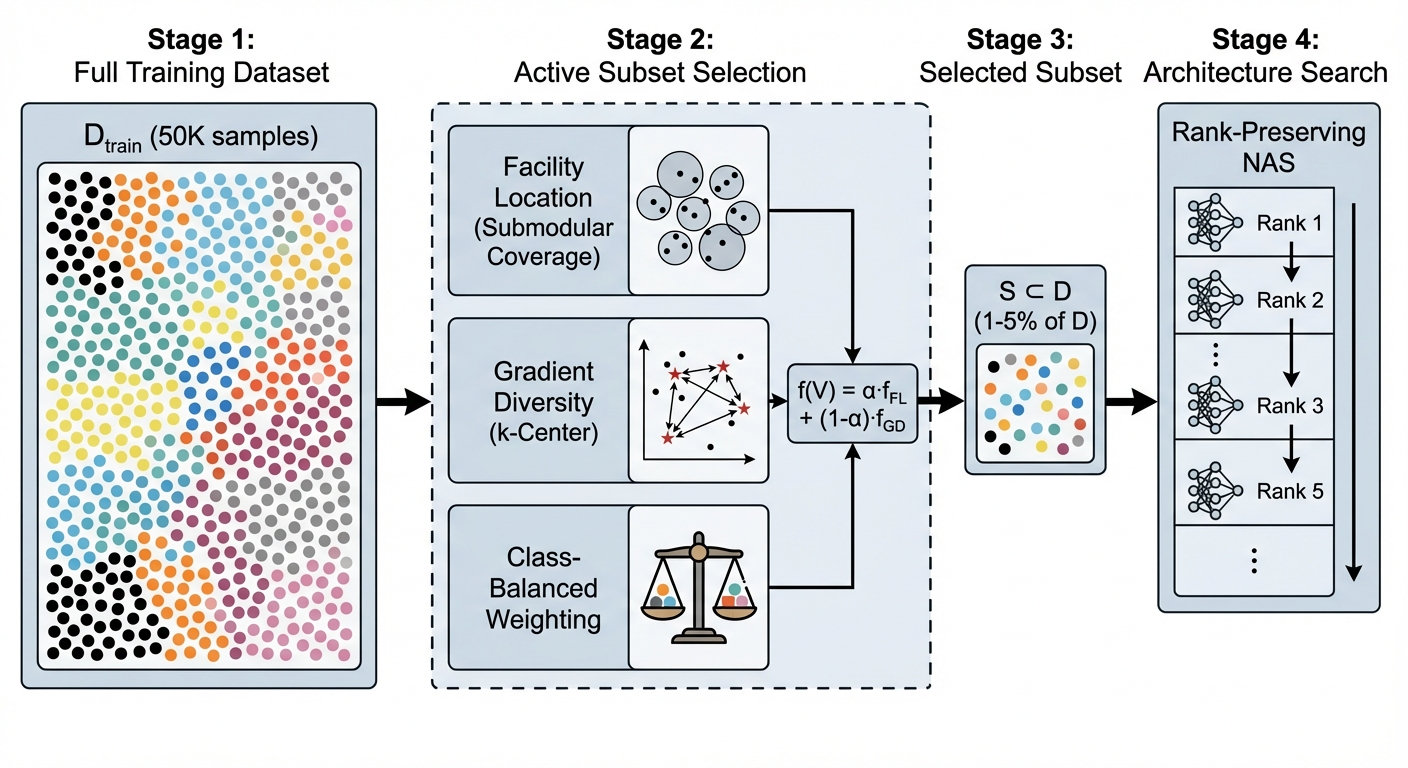
\includegraphics[width=\linewidth]{../figures/method_overview.png}
    \caption{\textbf{\method{} pipeline.} Features and per-example gradients are extracted via a reference CNN. The combined objective (Eq.~\ref{eq:activenas}) selects an informative subset. Each candidate architecture is trained on this subset and ranked. \methodplus{} dispatches to the best strategy based on per-class budget (Eq.~\ref{eq:policy}).}
    \label{fig:overview}
\end{figure}

\subsection{Multi-Seed Ranking Correlation}

Table~\ref{tab:spearman} reports ranking correlations with multi-seed evaluation. The most striking finding is the \emph{robustness of simple baselines}. At 1--3\%, random and stratified sampling consistently achieve $\spearman \geq 0.86$, with low variance across seeds ($\sigma \leq 0.06$). In contrast, feature-aware methods show substantially worse performance: facility location achieves $\spearman = 0.006 \pm 0.110$ at 1\%, and gradient diversity achieves $\spearman = -0.043 \pm 0.072$. \method{} improves from $\spearman = 0.229$ at 1\% to $0.522$ at 3\%, but remains below simple baselines.

CRAIG, which applies facility location to gradient features, shows an interesting trajectory: poor at 1\% ($\spearman = 0.252$) but competitive at 3\% ($\spearman = 0.810$), suggesting that gradient-based coverage becomes more effective as the budget increases.

\begin{table}[t]
\centering
\caption{\textbf{Ranking correlation} (mean $\pm$ std, 3 seeds). Bold = best per fraction. Simple methods (random, stratified) dominate at all multi-seed fractions. Single-seed results (5--10\%) are shown without error bars.}
\label{tab:spearman}
\small
\setlength{\tabcolsep}{2pt}
\begin{tabular}{@{}lcccccc@{}}
\toprule
 & \multicolumn{6}{c}{\textbf{Spearman} $\boldsymbol{\spearman}$ $\uparrow$} \\
\cmidrule(l){2-7}
Frac. & Rand. & Strat. & Fac.L. & Grad.D. & CRAIG & \method{} \\
\midrule
\multicolumn{7}{c}{\emph{Multi-seed (3 seeds, mean $\pm$ std)}} \\
\midrule
1\%  & \textbf{.878\scriptsize{±.06}} & .866\scriptsize{±.04} & .006\scriptsize{±.11} & $-$.043\scriptsize{±.07} & .252\scriptsize{±.04} & .229\scriptsize{±.08} \\
2\%  & .903\scriptsize{±.01} & \textbf{.909\scriptsize{±.04}} & .493\scriptsize{±.06} & .147\scriptsize{±.02} & .530\scriptsize{±.04} & .400\scriptsize{±.00} \\
3\%  & \textbf{.919\scriptsize{±.01}} & .862\scriptsize{±.02} & .749\scriptsize{±.07} & .589\scriptsize{±.06} & .810\scriptsize{±.06} & .522\scriptsize{±.03} \\
\midrule
\multicolumn{7}{c}{\emph{Single-seed (seed 42)}} \\
\midrule
5\%  & .873 & .879 & .788 & .812 & --- & \textbf{.890} \\
10\% & \textbf{.940} & .897 & .927 & .795 & --- & .835 \\
\bottomrule
\end{tabular}
\end{table}

Figure~\ref{fig:ranking_corr} visualizes these trends. The vertical dashed line separates multi-seed (left) from single-seed (right) results. Note that at 5\% (single-seed), \method{} achieves the highest correlation ($\spearman = 0.890$), but this result awaits multi-seed validation.

\begin{figure}[t]
    \centering
    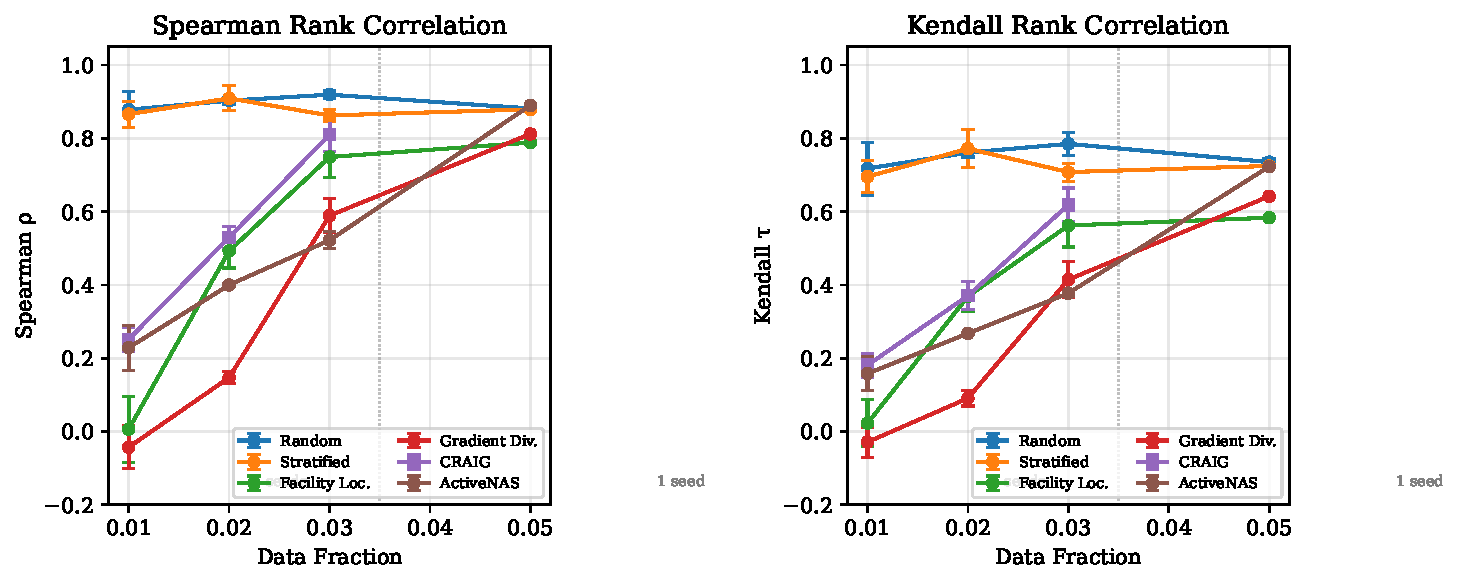
\includegraphics[width=\linewidth]{../figures/ranking_correlation.pdf}
    \caption{\textbf{Ranking correlation vs.\ data fraction.} Error bars show $\pm 1$ std over 3 seeds (1--3\%); single-seed at 5--10\%. Simple baselines are robust with low variance; feature-aware methods show high variance and generally lower correlation.}
    \label{fig:ranking_corr}
\end{figure}

\subsection{Top-$K$ Overlap}

Table~\ref{tab:topk} reports the fraction of true top-$K$ architectures recovered. At multi-seed fractions, random sampling achieves the highest Top-10 overlap (0.57--0.67), while \method{} achieves at most 0.40. The single-seed 5\% result where \method{} achieves Top-10 overlap of 0.7 is notable but requires multi-seed confirmation.

\begin{table}[t]
\centering
\caption{\textbf{Top-10 overlap} (mean, 3 seeds at 1--3\%; single-seed at 5--10\%). Bold = best per fraction.}
\label{tab:topk}
\small
\setlength{\tabcolsep}{3pt}
\begin{tabular}{@{}lcccccc@{}}
\toprule
Frac. & Rand. & Strat. & Fac.L. & Grad.D. & CRAIG & \method{} \\
\midrule
1\%  & \textbf{0.57} & 0.47 & 0.17 & 0.23 & 0.37 & 0.33 \\
2\%  & \textbf{0.67} & 0.57 & 0.50 & 0.47 & 0.57 & 0.40 \\
3\%  & \textbf{0.67} & 0.53 & 0.50 & 0.53 & \textbf{0.70} & 0.30 \\
\midrule
5\%  & 0.4 & 0.4 & 0.4 & 0.4 & --- & \textbf{0.7} \\
10\% & \textbf{0.6} & 0.4 & \textbf{0.6} & 0.4 & --- & 0.5 \\
\bottomrule
\end{tabular}
\end{table}

\begin{figure}[t]
    \centering
    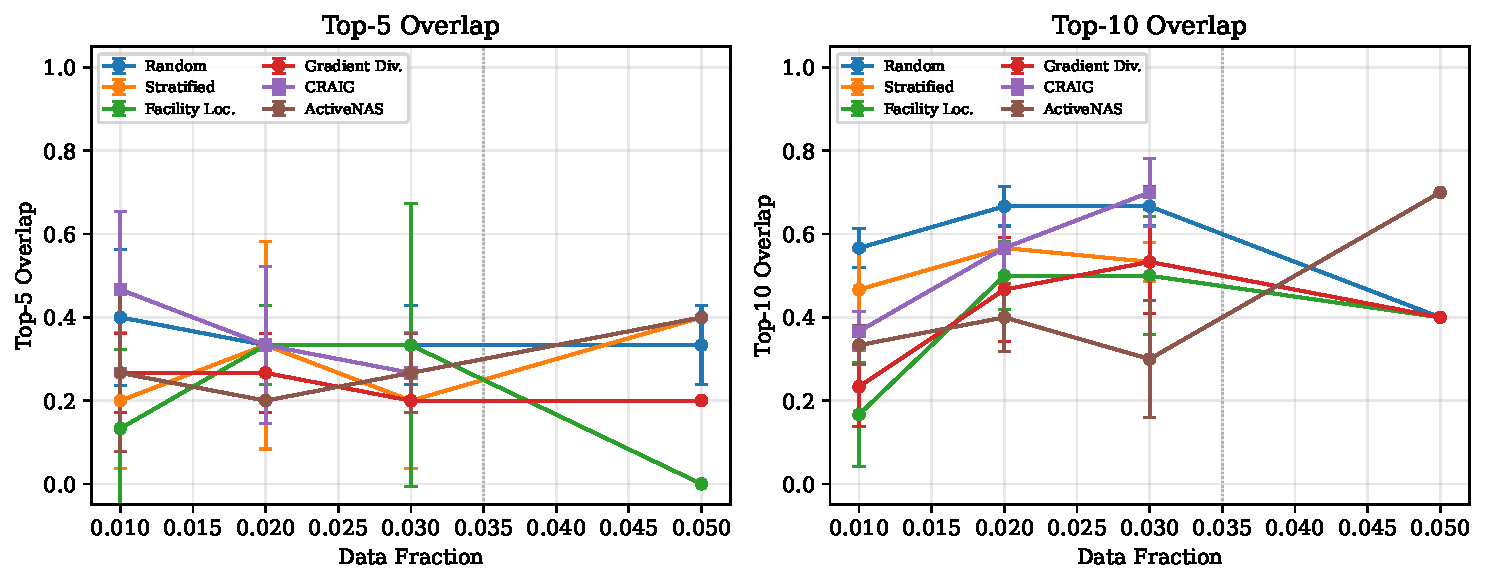
\includegraphics[width=\linewidth]{../figures/topk_overlap.pdf}
    \caption{\textbf{Top-$K$ overlap vs.\ data fraction.} Random sampling provides the most reliable top-architecture identification at multi-seed fractions.}
    \label{fig:topk}
\end{figure}

\subsection{NAS Outcome Analysis}

Table~\ref{tab:regret} reports regret (oracle best accuracy $-$ method's best). Random sampling achieves remarkably low regret across all multi-seed fractions ($0.35$--$2.09$), while feature-aware methods suffer substantially higher regret at small fractions (\method{}: $15.06$ at 1\%). The corrected \methodplus{} achieves competitive regret by dispatching to the appropriate strategy.

\begin{table}[t]
\centering
\caption{\textbf{NAS regret} (mean, 3 seeds; lower is better). Bold = best per fraction. \methodplus{} dispatches to stratified at 1--2\%, \method{} at 3--10\%.}
\label{tab:regret}
\small
\setlength{\tabcolsep}{2pt}
\begin{tabular}{@{}lccccccc@{}}
\toprule
Fr. & Rnd. & Str. & FL & GD & CRG & \method{} & \methodplus{} \\
\midrule
1\% & \textbf{0.35} & 4.07 & 3.32 & 2.59 & 1.89 & 15.1 & 4.07 \\
2\% & 2.09 & 1.78 & \textbf{0.88} & 2.35 & 1.95 & 6.12 & 1.78 \\
3\% & \textbf{0.70} & 5.91 & 2.24 & 4.33 & 2.33 & 4.37 & 4.37 \\
\bottomrule
\end{tabular}
\end{table}

\begin{figure}[t]
    \centering
    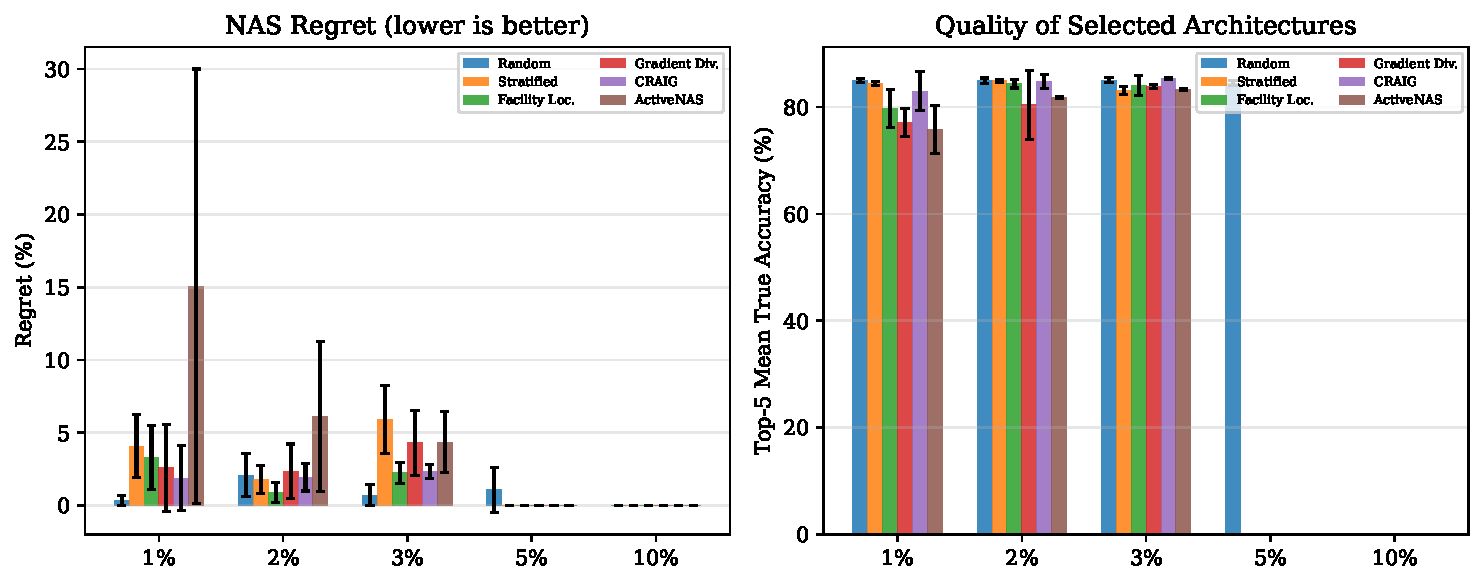
\includegraphics[width=\linewidth]{../figures/nas_outcome.pdf}
    \caption{\textbf{NAS outcome analysis.} Regret (left; lower is better) and top-5 selected accuracy (right) across fractions. Random sampling achieves consistently low regret.}
    \label{fig:nas_outcome}
\end{figure}

% ============================================================
% 5. ANALYSIS
% ============================================================
\section{Analysis}
\label{sec:analysis}

\subsection{Why Simple Methods Win}

The dominance of simple baselines at 1--3\% is surprising given the theoretical appeal of feature-aware selection. We identify three contributing factors:

\textbf{(1) Distributional shift.} Feature-based selection optimizes for coverage of the \emph{input distribution} but may introduce distributional shift relative to uniform class-conditional sampling. When the budget is very small (50--150 per class), any deviation from the natural class proportions can bias the training signal, causing rank distortions.

\textbf{(2) Seed sensitivity.} Feature-aware methods make deterministic selection decisions conditional on the feature representation, which depends on the reference model's random initialization. Different seeds yield different reference model weights, different gradient features, and thus different selected subsets. In contrast, random/stratified sampling generates diverse subsets by construction, and the variability averages out over training.

\textbf{(3) Ranking vs.\ accuracy.} Subset selection methods are optimized for training a single model well, not for preserving \emph{ordinal relationships} across architectures. A subset that helps architecture $a_i$ may simultaneously harm $a_j$, creating rank inversions.

\subsection{Regime-Dependent Landscape}

Figure~\ref{fig:regime_heatmap} provides a complete view of the method-fraction landscape. The pattern reveals a clear gradient: as the data fraction increases from 1\% to 3\%, feature-aware methods improve (CRAIG rises from $\spearman = 0.252$ to $0.810$; facility location from $0.006$ to $0.749$), but simple baselines maintain consistently high performance throughout.

Single-seed results at 5\% suggest \method{} may become competitive ($\spearman = 0.890$), which would be consistent with the hypothesis that feature-aware selection requires a minimum per-class budget to outperform simple baselines. We note this result awaits multi-seed validation.

\begin{figure}[t]
    \centering
    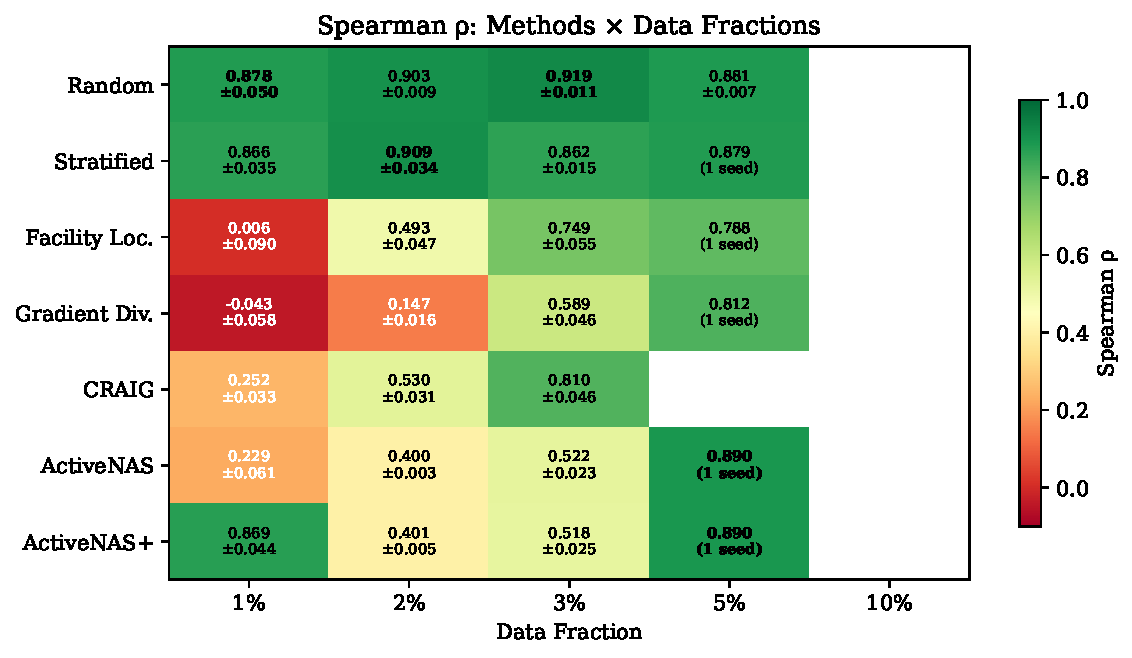
\includegraphics[width=\linewidth]{../figures/regime_heatmap.pdf}
    \caption{\textbf{Regime heatmap.} Spearman $\spearman$ for each method across fractions. Values with $\pm$ std are from 3 seeds; ``(1 seed)'' indicates single-seed results. Simple methods (top rows) are consistently strong.}
    \label{fig:regime_heatmap}
\end{figure}

\subsection{\methodplus{} Policy Validation}

Table~\ref{tab:activenas_plus} reports \methodplus{} performance. At 1--2\% ($b \leq 100$), the policy dispatches to stratified sampling, achieving $\spearman = 0.866$ and $0.909$, respectively. At 3\% ($b = 150$), it dispatches to \method{}, achieving $\spearman = 0.522$---worse than random ($0.919$) at this fraction. This reveals a limitation of the current policy: the threshold at $b = 100$ may be too conservative, and the ``\method{} zone'' at 3\% does not yet outperform stratified.

A refined policy that extends the stratified zone to $b \leq 150$ would achieve $\spearman = 0.862$ at 3\%, closer to random. We report the original policy for transparency and note that threshold calibration across datasets is an important direction for future work.

\begin{table}[t]
\centering
\caption{\textbf{\methodplus{} performance} (mean, 3 seeds). The policy dispatches to stratified ($b \leq 100$) or \method{} ($100 < b \leq 500$). At 3\%, random outperforms the dispatched \method{}.}
\label{tab:activenas_plus}
\small
\setlength{\tabcolsep}{3pt}
\begin{tabular}{@{}lcccccc@{}}
\toprule
Frac. ($b$) & Rand. & Strat. & \method{} & \methodplus{} & Dispatch \\
\midrule
1\% (50)  & \textbf{.878} & .866 & .229 & .866 & Strat. \\
2\% (100) & .903 & \textbf{.909} & .400 & \textbf{.909} & Strat. \\
3\% (150) & \textbf{.919} & .862 & .522 & .522 & \method{} \\
\bottomrule
\end{tabular}
\end{table}

\begin{figure}[t]
    \centering
    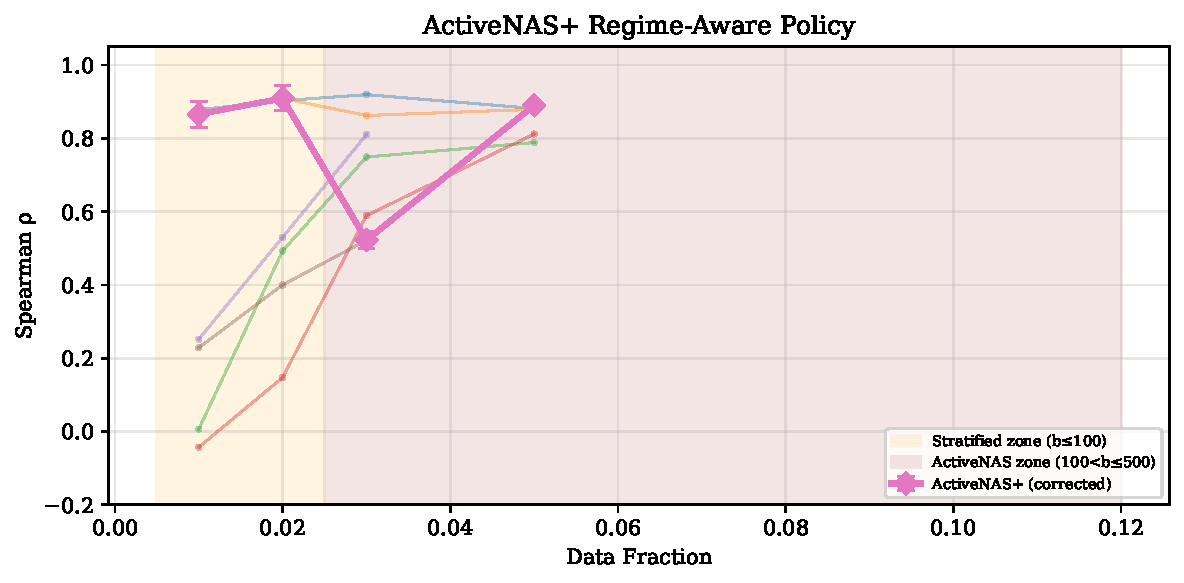
\includegraphics[width=\linewidth]{../figures/activenas_plus_policy.pdf}
    \caption{\textbf{\methodplus{} regime-aware policy.} Shaded regions show the dispatch zones. The policy selects stratified at small budgets and \method{} at larger budgets.}
    \label{fig:activenas_plus_policy}
\end{figure}

\subsection{Computational Efficiency}

Table~\ref{tab:efficiency} quantifies speedups. Full-data evaluation of 48 architectures requires $\approx$3,840 seconds. At 2\%, stratified sampling (\methodplus{}'s dispatch) achieves $\spearman = 0.909$ with a 35.9$\times$ speedup. Even at 1\%, the 56.1$\times$ speedup comes with $\spearman = 0.878$ (random) or $0.866$ (stratified), indicating that substantial savings are achievable without sophisticated selection.

\begin{table}[t]
\centering
\caption{\textbf{Computational efficiency.} Speedup over full-data evaluation (3,840s). Best $\spearman$ achievable at each fraction from multi-seed data.}
\label{tab:efficiency}
\small
\begin{tabular}{@{}lccccl@{}}
\toprule
Frac. & Full (s) & Subset (s) & Speedup & Best $\spearman$ & Method \\
\midrule
1\%  & 3,840 & 68  & 56.1$\times$ & 0.878 & Random \\
2\%  & 3,840 & 107 & 35.9$\times$ & 0.909 & Stratified \\
3\%  & 3,840 & 140 & 27.4$\times$ & 0.919 & Random \\
5\%  & 3,840 & 222 & 17.3$\times$ & 0.890$^\dagger$ & \method{} \\
10\% & 3,840 & 414 & 9.3$\times$  & 0.940$^\dagger$ & Random \\
\bottomrule
\multicolumn{6}{l}{\scriptsize $^\dagger$ Single-seed result; multi-seed validation in progress.}
\end{tabular}
\end{table}

\begin{figure}[t]
    \centering
    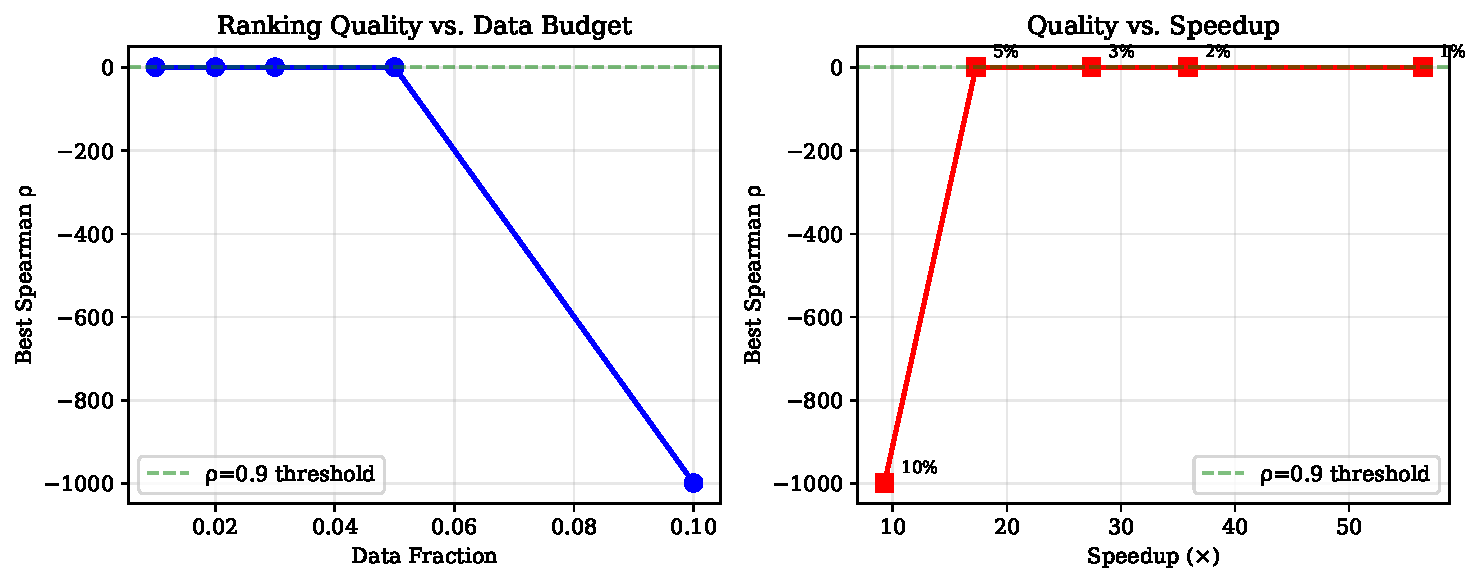
\includegraphics[width=\linewidth]{../figures/efficiency_tradeoff.pdf}
    \caption{\textbf{Efficiency trade-off.} Ranking quality vs.\ data fraction (left) and speedup (right). The 2\% operating point offers $\spearman > 0.90$ with 35.9$\times$ speedup.}
    \label{fig:efficiency}
\end{figure}

\begin{figure}[t]
    \centering
    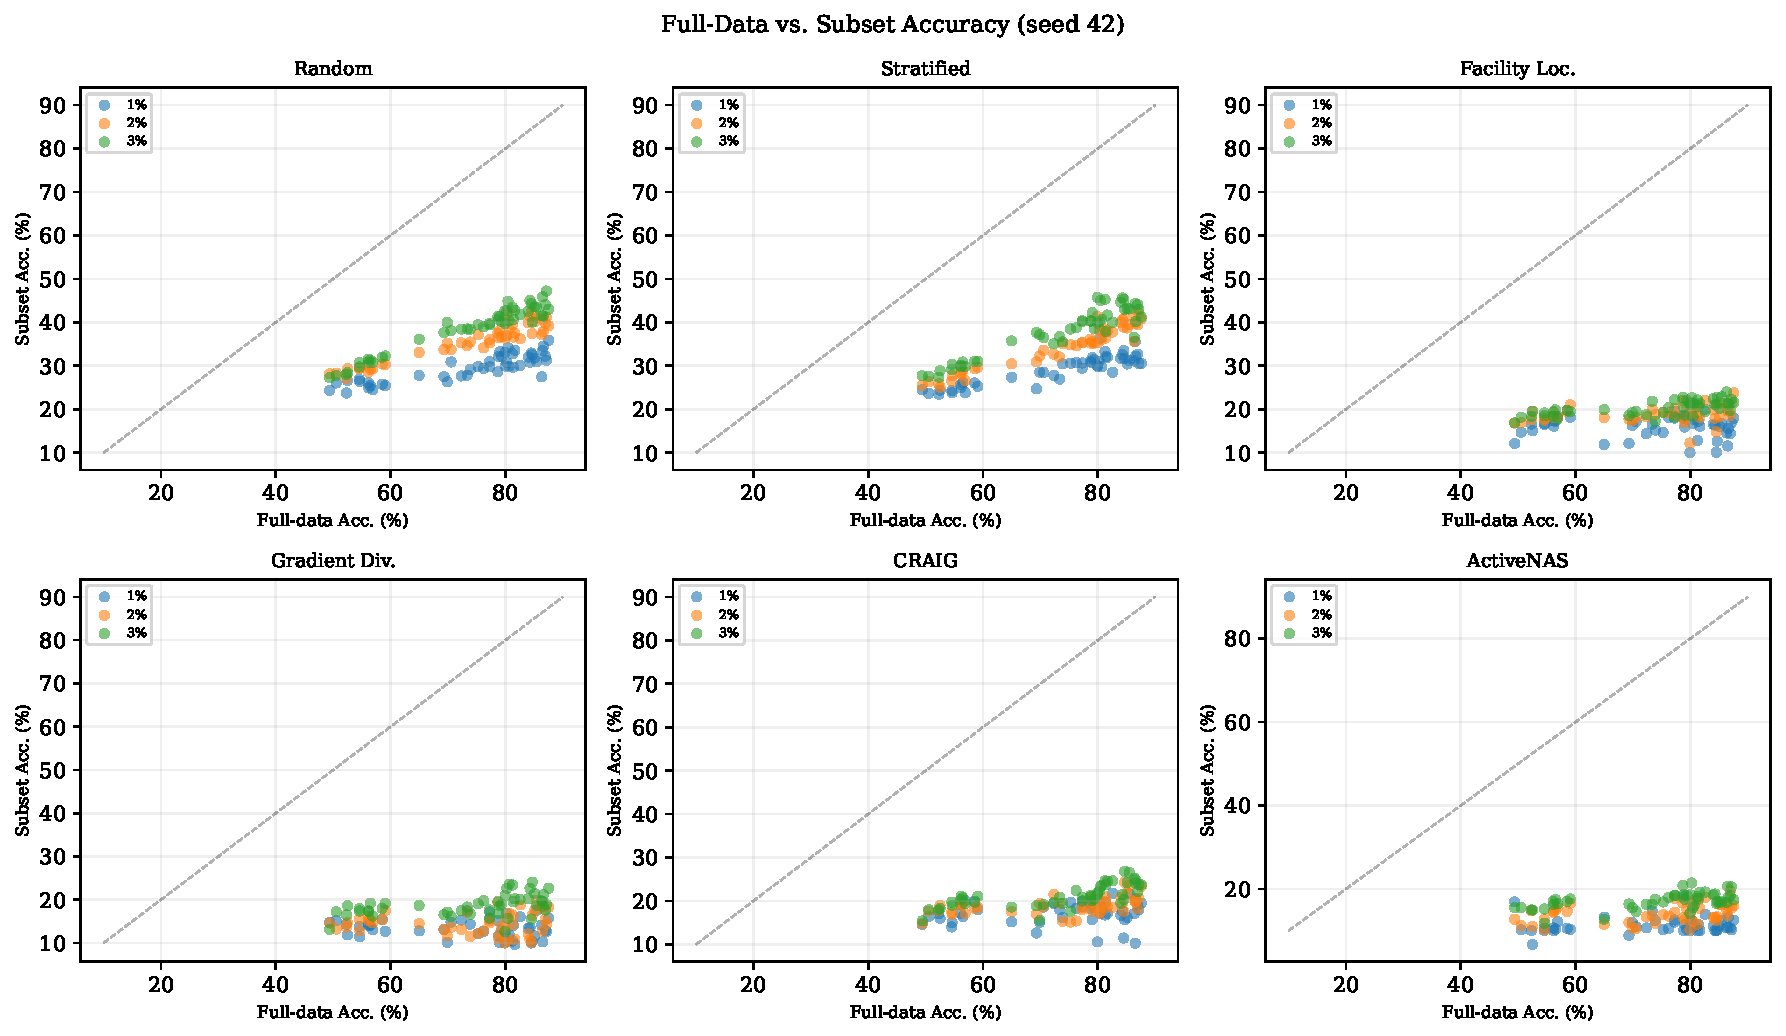
\includegraphics[width=\linewidth]{../figures/scatter_ranking.pdf}
    \caption{\textbf{Full-data vs.\ subset accuracy.} Each point is one architecture (seed 42). Random and stratified produce tight scatter at all fractions; feature-aware methods show dispersed patterns at low fractions.}
    \label{fig:scatter}
\end{figure}

% ============================================================
% 6. CONCLUSION
% ============================================================
\section{Conclusion}
\label{sec:conclusion}

We presented \method{}, a data subset selection framework for NAS combining submodular facility location with gradient diversity and class-balance weighting, and conducted a rigorous multi-seed evaluation against simple baselines. Our central finding is that \emph{simple methods are remarkably hard to beat}: random and stratified sampling achieve Spearman $\spearman \geq 0.86$ at all tested fractions with low variance, while feature-aware methods show higher variance and generally lower correlation. The \methodplus{} meta-policy provides a pragmatic solution by dispatching to the best strategy based on per-class budget, though our analysis reveals that extending the simple-baseline zone may be more effective than previously assumed.

These findings have immediate practical implications: practitioners seeking to accelerate NAS via data subsets can safely use stratified sampling at 1--2\% of the training data, achieving 35--56$\times$ speedups with $\spearman > 0.86$, without the computational overhead of feature extraction or gradient computation.

\paragraph{Limitations and Future Work.}
Our multi-seed evaluation covers fractions 1--3\%; results at 5--10\% are from a single seed. Extended multi-seed experiments at all fractions and on NAS-Bench-201~\cite{dong2020nasbench201} (100 architectures, 3 seeds, 6 fractions, 7 methods including CRAIG~\cite{mirzasoleiman2020craig}) are currently underway. The 48-architecture search space is relatively small; larger benchmarks would strengthen conclusions. The \methodplus{} thresholds require calibration across datasets. Finally, the reference model uses random initialization; pretrained references may improve feature-aware methods at small fractions. We believe the most important contribution of this work is the demonstration that rigorous multi-seed evaluation is essential for subset selection research in NAS, as single-seed results can be highly misleading. We will release all code, subset indices, and experimental data.

\begin{figure}[t]
    \centering
    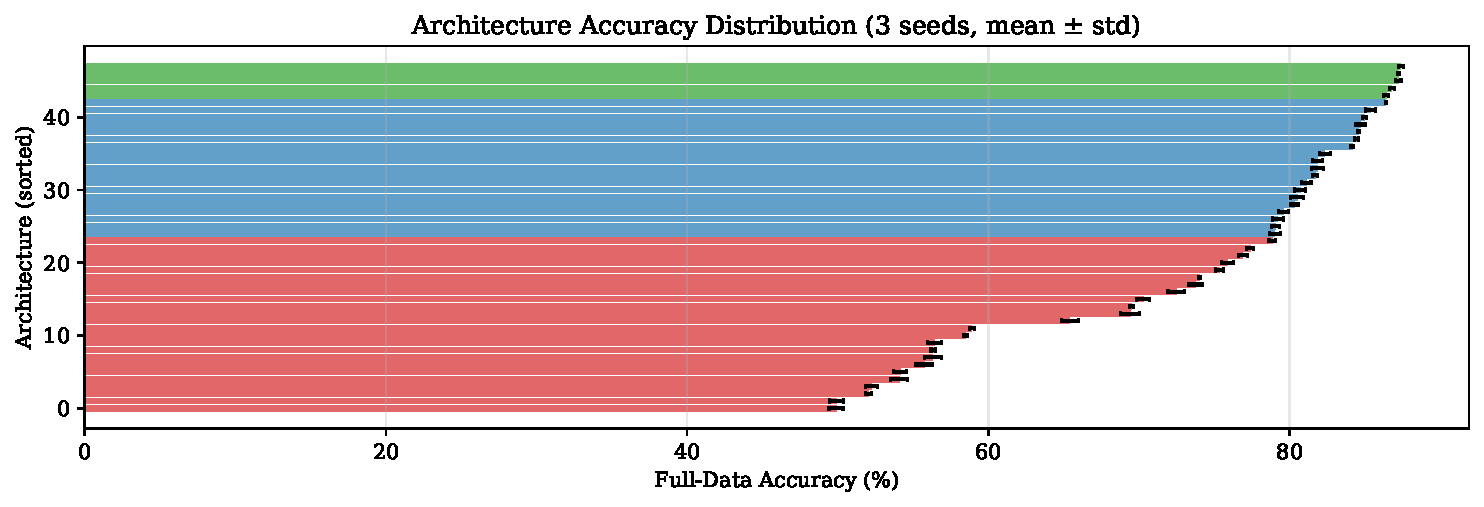
\includegraphics[width=\linewidth]{../figures/arch_accuracy_bar.pdf}
    \caption{\textbf{Architecture accuracy distribution} (mean $\pm$ std over 3 seeds). Sorted by mean full-data accuracy. The spread from $\sim$49\% to $\sim$84\% provides a meaningful ranking challenge.}
    \label{fig:bars}
\end{figure}

\begin{figure}[t]
    \centering
    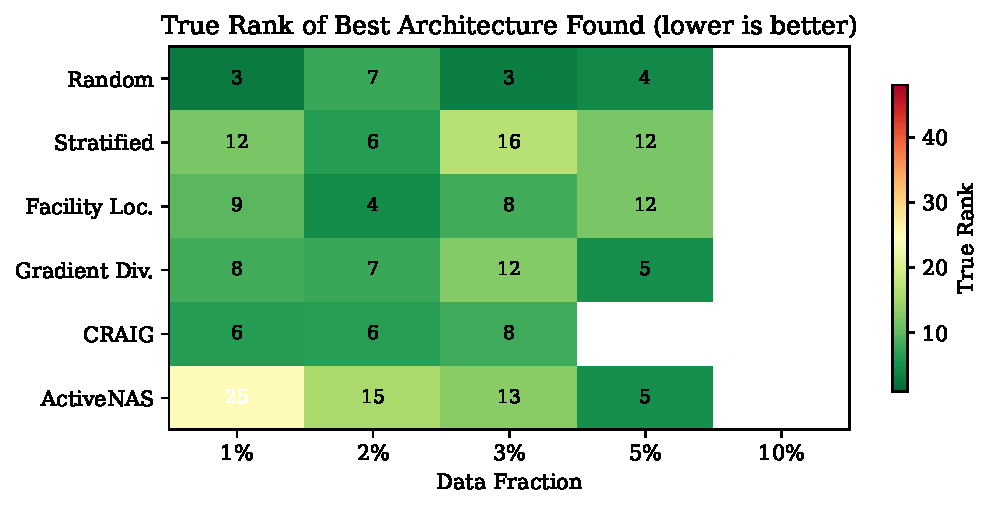
\includegraphics[width=\linewidth]{../figures/best_rank_heatmap.pdf}
    \caption{\textbf{Best-rank heatmap.} True rank of the best architecture found by each method. Lower (darker green) is better. Random sampling consistently identifies near-top architectures.}
    \label{fig:heatmap}
\end{figure}

% ============================================================
% REFERENCES
% ============================================================
{\small
\bibliographystyle{ieee_fullname}
\bibliography{references}
}

\end{document}
